
%% bare_conf.tex
%% V1.4b
%% 2015/08/26
%% by Michael Shell
%% See:
%% http://www.michaelshell.org/
%% for current contact information.
%%
%% This is a skeleton file demonstrating the use of IEEEtran.cls
%% (requires IEEEtran.cls version 1.8b or later) with an IEEE
%% conference paper.
%%
%% Support sites:
%% http://www.michaelshell.org/tex/ieeetran/
%% http://www.ctan.org/pkg/ieeetran
%% and
%% http://www.ieee.org/

%%*************************************************************************
%% Legal Notice:
%% This code is offered as-is without any warranty either expressed or
%% implied; without even the implied warranty of MERCHANTABILITY or
%% FITNESS FOR A PARTICULAR PURPOSE!
%% User assumes all risk.
%% In no event shall the IEEE or any contributor to this code be liable for
%% any damages or losses, including, but not limited to, incidental,
%% consequential, or any other damages, resulting from the use or misuse
%% of any information contained here.
%%
%% All comments are the opinions of their respective authors and are not
%% necessarily endorsed by the IEEE.
%%
%% This work is distributed under the LaTeX Project Public License (LPPL)
%% ( http://www.latex-project.org/ ) version 1.3, and may be freely used,
%% distributed and modified. A copy of the LPPL, version 1.3, is included
%% in the base LaTeX documentation of all distributions of LaTeX released
%% 2003/12/01 or later.
%% Retain all contribution notices and credits.
%% ** Modified files should be clearly indicated as such, including  **
%% ** renaming them and changing author support contact information. **
%%*************************************************************************


% *** Authors should verify (and, if needed, correct) their LaTeX system  ***
% *** with the testflow diagnostic prior to trusting their LaTeX platform ***
% *** with production work. The IEEE's font choices and paper sizes can   ***
% *** trigger bugs that do not appear when using other class files.       ***                          ***
% The testflow support page is at:
% http://www.michaelshell.org/tex/testflow/



\documentclass[a4paper,conference]{IEEEtran}
% Some Computer Society conferences also require the compsoc mode option,
% but others use the standard conference format.
%
% If IEEEtran.cls has not been installed into the LaTeX system files,
% manually specify the path to it like:
% \documentclass[conference]{../sty/IEEEtran}





% Some very useful LaTeX packages include:
% (uncomment the ones you want to load)


% *** MISC UTILITY PACKAGES ***
%
%\usepackage{ifpdf}
% Heiko Oberdiek's ifpdf.sty is very useful if you need conditional
% compilation based on whether the output is pdf or dvi.
% usage:
% \ifpdf
%   % pdf code
% \else
%   % dvi code
% \fi
% The latest version of ifpdf.sty can be obtained from:
% http://www.ctan.org/pkg/ifpdf
% Also, note that IEEEtran.cls V1.7 and later provides a builtin
% \ifCLASSINFOpdf conditional that works the same way.
% When switching from latex to pdflatex and vice-versa, the compiler may
% have to be run twice to clear warning/error messages.






% *** CITATION PACKAGES ***
%
%\usepackage{cite}
% cite.sty was written by Donald Arseneau
% V1.6 and later of IEEEtran pre-defines the format of the cite.sty package
% \cite{} output to follow that of the IEEE. Loading the cite package will
% result in citation numbers being automatically sorted and properly
% "compressed/ranged". e.g., [1], [9], [2], [7], [5], [6] without using
% cite.sty will become [1], [2], [5]--[7], [9] using cite.sty. cite.sty's
% \cite will automatically add leading space, if needed. Use cite.sty's
% noadjust option (cite.sty V3.8 and later) if you want to turn this off
% such as if a citation ever needs to be enclosed in parenthesis.
% cite.sty is already installed on most LaTeX systems. Be sure and use
% version 5.0 (2009-03-20) and later if using hyperref.sty.
% The latest version can be obtained at:
% http://www.ctan.org/pkg/cite
% The documentation is contained in the cite.sty file itself.


\usepackage{graphics} % for pdf, bitmapped graphics files
\usepackage[]{algorithm2e}
\usepackage{epsfig} % for postscript graphics files
\usepackage{mathptmx} % assumes new font selection scheme installed
%\usepackage{times} % assumes new font selection scheme installed
\usepackage{amsmath} % assumes amsmath package installed
\usepackage{balance}
%\usepackage{amssymb}  % assumes amsmath package installed
\usepackage{multirow}



% *** GRAPHICS RELATED PACKAGES ***
%
\ifCLASSINFOpdf
  % \usepackage[pdftex]{graphicx}
  % declare the path(s) where your graphic files are
  % \graphicspath{{../pdf/}{../jpeg/}}
  % and their extensions so you won't have to specify these with
  % every instance of \includegraphics
  % \DeclareGraphicsExtensions{.pdf,.jpeg,.png}
\else
  % or other class option (dvipsone, dvipdf, if not using dvips). graphicx
  % will default to the driver specified in the system graphics.cfg if no
  % driver is specified.
  % \usepackage[dvips]{graphicx}
  % declare the path(s) where your graphic files are
  % \graphicspath{{../eps/}}
  % and their extensions so you won't have to specify these with
  % every instance of \includegraphics
  % \DeclareGraphicsExtensions{.eps}
\fi
% graphicx was written by David Carlisle and Sebastian Rahtz. It is
% required if you want graphics, photos, etc. graphicx.sty is already
% installed on most LaTeX systems. The latest version and documentation
% can be obtained at:
% http://www.ctan.org/pkg/graphicx
% Another good source of documentation is "Using Imported Graphics in
% LaTeX2e" by Keith Reckdahl which can be found at:
% http://www.ctan.org/pkg/epslatex
%
% latex, and pdflatex in dvi mode, support graphics in encapsulated
% postscript (.eps) format. pdflatex in pdf mode supports graphics
% in .pdf, .jpeg, .png and .mps (metapost) formats. Users should ensure
% that all non-photo figures use a vector format (.eps, .pdf, .mps) and
% not a bitmapped formats (.jpeg, .png). The IEEE frowns on bitmapped formats
% which can result in "jaggedy"/blurry rendering of lines and letters as
% well as large increases in file sizes.
%
% You can find documentation about the pdfTeX application at:
% http://www.tug.org/applications/pdftex





% *** MATH PACKAGES ***
%
%\usepackage{amsmath}
% A popular package from the American Mathematical Society that provides
% many useful and powerful commands for dealing with mathematics.
%
% Note that the amsmath package sets \interdisplaylinepenalty to 10000
% thus preventing page breaks from occurring within multiline equations. Use:
%\interdisplaylinepenalty=2500
% after loading amsmath to restore such page breaks as IEEEtran.cls normally
% does. amsmath.sty is already installed on most LaTeX systems. The latest
% version and documentation can be obtained at:
% http://www.ctan.org/pkg/amsmath





% *** SPECIALIZED LIST PACKAGES ***
%
%\usepackage{algorithmic}
% algorithmic.sty was written by Peter Williams and Rogerio Brito.
% This package provides an algorithmic environment fo describing algorithms.
% You can use the algorithmic environment in-text or within a figure
% environment to provide for a floating algorithm. Do NOT use the algorithm
% floating environment provided by algorithm.sty (by the same authors) or
% algorithm2e.sty (by Christophe Fiorio) as the IEEE does not use dedicated
% algorithm float types and packages that provide these will not provide
% correct IEEE style captions. The latest version and documentation of
% algorithmic.sty can be obtained at:
% http://www.ctan.org/pkg/algorithms
% Also of interest may be the (relatively newer and more customizable)
% algorithmicx.sty package by Szasz Janos:
% http://www.ctan.org/pkg/algorithmicx




% *** ALIGNMENT PACKAGES ***
%
%\usepackage{array}
% Frank Mittelbach's and David Carlisle's array.sty patches and improves
% the standard LaTeX2e array and tabular environments to provide better
% appearance and additional user controls. As the default LaTeX2e table
% generation code is lacking to the point of almost being broken with
% respect to the quality of the end results, all users are strongly
% advised to use an enhanced (at the very least that provided by array.sty)
% set of table tools. array.sty is already installed on most systems. The
% latest version and documentation can be obtained at:
% http://www.ctan.org/pkg/array


% IEEEtran contains the IEEEeqnarray family of commands that can be used to
% generate multiline equations as well as matrices, tables, etc., of high
% quality.




% *** SUBFIGURE PACKAGES ***
%\ifCLASSOPTIONcompsoc
%  \usepackage[caption=false,font=normalsize,labelfont=sf,textfont=sf]{subfig}
%\else
%  \usepackage[caption=false,font=footnotesize]{subfig}
%\fi
% subfig.sty, written by Steven Douglas Cochran, is the modern replacement
% for subfigure.sty, the latter of which is no longer maintained and is
% incompatible with some LaTeX packages including fixltx2e. However,
% subfig.sty requires and automatically loads Axel Sommerfeldt's caption.sty
% which will override IEEEtran.cls' handling of captions and this will result
% in non-IEEE style figure/table captions. To prevent this problem, be sure
% and invoke subfig.sty's "caption=false" package option (available since
% subfig.sty version 1.3, 2005/06/28) as this is will preserve IEEEtran.cls
% handling of captions.
% Note that the Computer Society format requires a larger sans serif font
% than the serif footnote size font used in traditional IEEE formatting
% and thus the need to invoke different subfig.sty package options depending
% on whether compsoc mode has been enabled.
%
% The latest version and documentation of subfig.sty can be obtained at:
% http://www.ctan.org/pkg/subfig




% *** FLOAT PACKAGES ***
%
%\usepackage{fixltx2e}
% fixltx2e, the successor to the earlier fix2col.sty, was written by
% Frank Mittelbach and David Carlisle. This package corrects a few problems
% in the LaTeX2e kernel, the most notable of which is that in current
% LaTeX2e releases, the ordering of single and double column floats is not
% guaranteed to be preserved. Thus, an unpatched LaTeX2e can allow a
% single column figure to be placed prior to an earlier double column
% figure.
% Be aware that LaTeX2e kernels dated 2015 and later have fixltx2e.sty's
% corrections already built into the system in which case a warning will
% be issued if an attempt is made to load fixltx2e.sty as it is no longer
% needed.
% The latest version and documentation can be found at:
% http://www.ctan.org/pkg/fixltx2e


%\usepackage{stfloats}
% stfloats.sty was written by Sigitas Tolusis. This package gives LaTeX2e
% the ability to do double column floats at the bottom of the page as well
% as the top. (e.g., "\begin{figure*}[!b]" is not normally possible in
% LaTeX2e). It also provides a command:
%\fnbelowfloat
% to enable the placement of footnotes below bottom floats (the standard
% LaTeX2e kernel puts them above bottom floats). This is an invasive package
% which rewrites many portions of the LaTeX2e float routines. It may not work
% with other packages that modify the LaTeX2e float routines. The latest
% version and documentation can be obtained at:
% http://www.ctan.org/pkg/stfloats
% Do not use the stfloats baselinefloat ability as the IEEE does not allow
% \baselineskip to stretch. Authors submitting work to the IEEE should note
% that the IEEE rarely uses double column equations and that authors should try
% to avoid such use. Do not be tempted to use the cuted.sty or midfloat.sty
% packages (also by Sigitas Tolusis) as the IEEE does not format its papers in
% such ways.
% Do not attempt to use stfloats with fixltx2e as they are incompatible.
% Instead, use Morten Hogholm'a dblfloatfix which combines the features
% of both fixltx2e and stfloats:
%
% \usepackage{dblfloatfix}
% The latest version can be found at:
% http://www.ctan.org/pkg/dblfloatfix




% *** PDF, URL AND HYPERLINK PACKAGES ***
%
%\usepackage{url}
% url.sty was written by Donald Arseneau. It provides better support for
% handling and breaking URLs. url.sty is already installed on most LaTeX
% systems. The latest version and documentation can be obtained at:
% http://www.ctan.org/pkg/url
% Basically, \url{my_url_here}.




% *** Do not adjust lengths that control margins, column widths, etc. ***
% *** Do not use packages that alter fonts (such as pslatex).         ***
% There should be no need to do such things with IEEEtran.cls V1.6 and later.
% (Unless specifically asked to do so by the journal or conference you plan
% to submit to, of course. )


% correct bad hyphenation here
\hyphenation{op-tical net-works semi-conduc-tor}


\begin{document}
%
% paper title
% Titles are generally capitalized except for words such as a, an, and, as,
% at, but, by, for, in, nor, of, on, or, the, to and up, which are usually
% not capitalized unless they are the first or last word of the title.
% Linebreaks \\ can be used within to get better formatting as desired.
% Do not put math or special symbols in the title.
\title{Learning from learners: Adapting Reinforcement Learning Agents to be Competitive in a Card Game.}


% author names and affiliations
% use a multiple column layout for up to three different
% affiliations
\author{\IEEEauthorblockN{Pablo Barros, Ana Tanevska and Alessandra Sciutti}
\IEEEauthorblockA{Cognitive Architecture for \\Collaborative Technologies(CONTACT) Unit \\Istituto Italiano di Tecnologia\\ Genova, Italy\\
Emails: \{pablo.avesdebarros, ana.tanevska, alessandra.sciutti\}@iit.it}
% \and
% \IEEEauthorblockN{Ana Tanevska}
% \IEEEauthorblockA{Cognitive Architecture for \\Collaborative Technologies\\ (CONTACT) Unit \\Istituto Italiano di Tecnologia\\ Genova, Italy
% Email: ana.tanevska@iit.it}
% \and
% \IEEEauthorblockN{Alessandra Sciutti}
% \IEEEauthorblockA{Cognitive Architecture for \\Collaborative Technologies\\ (CONTACT)\ Unit \\Istituto Italiano di Tecnologia\\ Genova, Italy
% Email: alessandra.sciutti@iit.it}

}

% conference papers do not typically use \thanks and this command
% is locked out in conference mode. If really needed, such as for
% the acknowledgment of grants, issue a \IEEEoverridecommandlockouts
% after \documentclass

% for over three affiliations, or if they all won't fit within the width
% of the page, use this alternative format:
%
%\author{\IEEEauthorblockN{Michael Shell\IEEEauthorrefmark{1},
%Homer Simpson\IEEEauthorrefmark{2},
%James Kirk\IEEEauthorrefmark{3},
%Montgomery Scott\IEEEauthorrefmark{3} and
%Eldon Tyrell\IEEEauthorrefmark{4}}
%\IEEEauthorblockA{\IEEEauthorrefmark{1}School of Electrical and Computer Engineering\\
%Georgia Institute of Technology,
%Atlanta, Georgia 30332--0250\\ Email: see http://www.michaelshell.org/contact.html}
%\IEEEauthorblockA{\IEEEauthorrefmark{2}Twentieth Century Fox, Springfield, USA\\
%Email: homer@thesimpsons.com}
%\IEEEauthorblockA{\IEEEauthorrefmark{3}Starfleet Academy, San Francisco, California 96678-2391\\
%Telephone: (800) 555--1212, Fax: (888) 555--1212}
%\IEEEauthorblockA{\IEEEauthorrefmark{4}Tyrell Inc., 123 Replicant Street, Los Angeles, California 90210--4321}}




% use for special paper notices
%\IEEEspecialpapernotice{(Invited Paper)}




% make the title area
\maketitle

% As a general rule, do not put math, special symbols or citations
% in the abstract
\begin{abstract}
The abstract goes here.
\end{abstract}

% no keywords




% For peer review papers, you can put extra information on the cover
% page as needed:
% \ifCLASSOPTIONpeerreview
% \begin{center} \bfseries EDICS Category: 3-BBND \end{center}
% \fi
%
% For peerreview papers, this IEEEtran command inserts a page break and
% creates the second title. It will be ignored for other modes.
\IEEEpeerreviewmaketitle



\section{Introduction}

% Learning how to adapt to complex and dynamic environments is one of the most important factors that contribute to our intelligence. Translating this characteristic into artificial agents proved to be a difficult task \cite{mnih2015human, hessel2018rainbow, henderson2018deep}. The mapping between actions and environmental rewards became a very popular solution for creating autonomous artificial agents that do not rely on explicit supervision, in particular with the last two decades of development on reinforcement learning. Such agents usually embed different policy learning mechanisms that allow them to develop decision-making strategies which are, in some cases, unexpected or unknown by humans \cite{wang2016does, silver2018general}. 

% With the recent interest in reinforcement learning caused by the development of deep reinforcement learning techniques \cite{mnih2013playing}, novel methods, mechanisms, and scenarios were developed in recent years. Such mechanisms allow the agent to process highly complex scenarios, such as high-resolution raw images \cite{lillicrap2015continuous}, in an end-to-end learning manner reducing the need for strong and well-defined prior knowledge.

% The proliferation of different reinforcement learning techniques contributes to the incredible increase on popularity that such research field had recently, which as a consequence p

With the current interest in reinforcement learning caused by the development of deep reinforcement learning techniques \cite{mnih2013playing}, novel methods, mechanisms, and scenarios have been developed in recent years. Such mechanisms allow the agent to process highly complex scenarios and data, such as high-resolution raw images \cite{lillicrap2015continuous}, in an end-to-end learning manner reducing the need for strong and well-defined prior knowledge. With such popularity, the applications of reinforcement learning are leaving the traditional simple scenarios. In recent cases, reinforcement learning agents have been used for guiding autonomous cars \cite{sallab2017deep, isele2018navigating}, predicting the stock exchange impact \cite{ponomarev2019using, meng2019reinforcement}, and coordinating a swarm of robots to protect the environment \cite{haksar2018distributed, yu2018reinforcement}. Most of these solutions, although having real-world-inspired scenarios, focus on a direct space-action-reward mapping between the agent's action and the environment state. That translates to agents that can adapt to dynamic scenarios, but, in most cases, when choosing an action do not take into consideration how other agents can affect the state of the scenario. In this regard, competitive reinforcement learning is still behind the mainstream applications and demonstrations of the last years.

In competitive scenarios, the agents have to learn decisions that a) maximize their goal, and b) minimize their adversaries' goals. Besides dealing with complex scenarios, they usually have to deal with the dynamics between the agents themselves. The most common applications scenarios for competitive reinforcement learning involve multi-agent simulations, such as multiple autonomous vehicles \cite{fridman2018deeptraffic}, life-simulation/resources gathering \cite{xu2018hierarchical}, pursuer/pursued scenarios \cite{wang2019competitive}), and multi-player games \cite{mckenzie2017competitive}. 

In this direction, the increased development and popular interest in deep reinforcement learning has contributed to the design of a few competitive learning solutions. The implementation of a counterfactual thinking solution \cite{wang2019competitive}, based on the classic psychological phenomenon, obtained a good performance on a simple multi-agent water world scenario \cite{gupta2017cooperative}. This scenario consisted of a life-simulation where the agents try to compete for resources. Although the model in question presented good overall performance, it increased the complexity of the decision making by adding a counterfactual policy network within the agent's internal state. This network showed to be sensitive to different hyperparameters and thus hard to scale to more complex scenarios.

Another proposed scenario of greater success has been the recent implementation of a general multi-agent actor-critic model for cooperative and competitive scenarios \cite{tampuu2017multiagent}. This model introduced novel implementations for Deep Q-learning that allowed it to be used in different competitive and cooperative scenarios. Additionally, for the competitive scenarios the authors proposed a novel training mechanism that allowed them to use the information of other agent's actions towards a general and centralized learning behavior. This presents an effective way of learning competitive actions, but it is rather centralized as the learner must have total control of the environment to be able to update the agents. Moreover, most of these scenarios are evaluated using very limited simulations of real-world events and most of the time do not scale well to real-world problems \cite{hernandez2019survey}. 

To assess how popular reinforcement learning methods behave in a real-world competitive scenario, in this paper we propose a broad study on how different reinforcement learning agents learn and behave when deployed in such an environment. We investigate how three popular reinforcement learning models (Deep Q-Learning - DQL \cite{van2016deep}, Advantage Actor-Critic - A2C \cite{mnih2016asynchronous}, and Proximal Policy Optimization - PPO \cite{schulman2017proximal}) can learn a competitive card game, and evaluate how their emerged behavior affect their own decisions towards winning the game. By focusing on these three implementations, we aim to provide the training, analysis and performance baseline for the competitive Chef's Hat card game \cite{barros2020food}, without the need of a centralized learner or overly-complex solutions. Our goal is to understand how these established implementations behave in a real-world inspired competitive scenario.

To maintain our scenario as close to real-world as possible, we implement in full the Chef's Hat card game, which has been designed to be used in Human-Robot Interactions (HRI). The game contains specific mechanics that allow complex dynamics between the players to be used in the development of a winning game strategy. We use the OpenAI Gym-based Chef's Hat simulation environment \cite{barros2020chef} to emulate, in a 1:1 scale, all the possible game mechanics. A card game scenario allows us to have a naturally-constrained environment and yet obtain responses that are the same as the real-world counter-part application. It additionally helps us to better understand the decision-making process of the agents and to better illustrate the strategies learned by each agent and how they affect each other.

For each of the three reinforcement learning methods, we introduce adaptations to the learning mechanisms of each agent, including a novel greedy policy for action selection. We perform three main competitive learning tasks: first, each of these agents is trained against random agents, to evaluate their capability to learn a game strategy. Second, we deploy a self-play routine that allows each agent to further improve its strategies by playing with evolving versions of itself. Third, once all the agents are trained, we choose the best of them and perform an inter-method competition, where the best agents of each learning method play against each other.

We compare the performance of these agents by measuring two main metrics: their averaged reward per game, and the number of wins they have in a series of games. To better understand and explain their learned strategies, we also evaluate their action-selection behavior over time, their ability to adhere to the rules of the game, and their capability of disrupting other agents by forcing them to change their action-selection behavior.


\section{Learning to be Competitive}

\begin{figure}
\begin{center}
  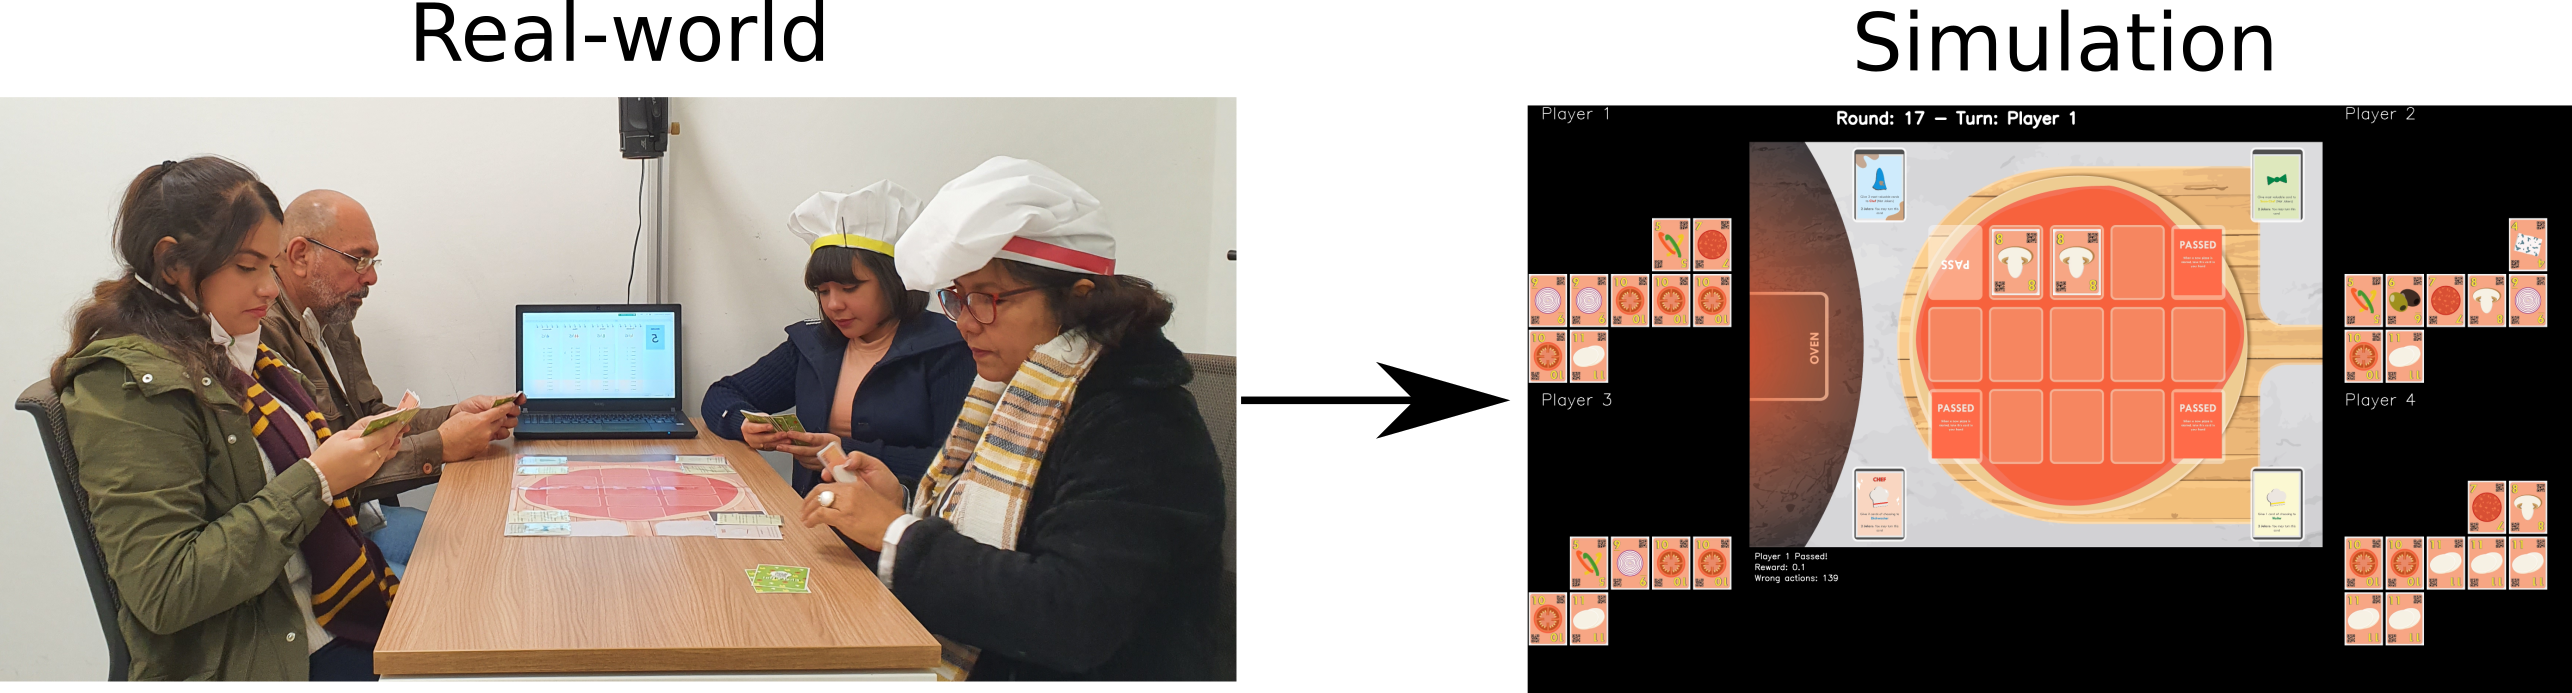
\includegraphics[width=1\linewidth]{realWorld-Simulation.png}
\end{center}
  \caption{We use the Chef's Hat simulation environment \cite{barros2020chef} to have a 1:1 reproduction of the real card game.}
\label{fig:gameExample}
\end{figure}

The concept of competitiveness can be modeled in many different manners. At first, the most important metric for an agent to be competitive is to define the overall environment goal. In our card game scenario, we define the overall metric as winning as many games as possible. This gives each agent a clear goal and allows us to observe how this clear goal affects the agent's behavior while playing the game, and which strategies emerge.

To be able to observe and understand the emerging strategies, we implement the Chef's Hat card game \cite{barros2020food} through the OpenAI-based simulation environment \cite{barros2020chef}, illustrated at Figure \ref{fig:gameExample}. This card game represents a controllable action-perception cycle, where each player can only perform a restricted set of actions, and we can directly measure the impact of each action within the game state and the formation of player's strategy. Furthermore, it allows each player to behave as organically as possible, given the in-game constraints, and allows for a naturally-controllable real-world scenario. 

% In our experiments with artificial agents, we use the Chef's Hat OpenAI-based simulation environment \cite{barros2020chef}, which implements the game in a 1:1 relation. It includes all the complex game mechanics, and allow us to represent all the interaction dynamics.


\subsection{Chef's Hat Card Game Mechanics}

Chef's Hat is played by four players and has as a theme a kitchen environment. The game was designed, implemented and validated in a way to allow Human-Robot Interaction experiments to be conducted, where one player can be replaced by a robot without changing the game rules or dynamics. This contributes to the development of virtual agents playing the game in the same manner as humans, and thus, the simulation allows a true representation of the real-world game scenario.

The game is composed of a role-based hierarchy: each player can either be a Chef, a Sous-Chef, a Waiter, or a Dishwasher. The objective of the players is to be the first one to get rid of their ingredient cards and become the Chef. Each game is described in details at Algorithm \ref{alg:ChefsHat}). The player which was the most times the Chef is considered the overall winner of the entire game.


\begin{algorithm}
 Shuffle the deck; \\
Deal an equal amount of cards per player; \\
  Exchange roles; \\
  Exchange cards; \\
   \If{special action is evoked}
  {
    Do special action;
  }
  
 \State $FirstPlayer\gets Has golden 11$\\
 $FirstPlayer$ discard cards. \\
 
 \While{not end of the game}{
  \For{ each player}{

      \eIf{player can, and want, to discard}{
       discard cards\;
       }{
        pass\;
      }
      \If{All players passed}
      {
        Make the pizza;
         \State $FirstPlayer\gets Last player to discard$\\
      }
        \If{All players finished}
      {
        End of game.
      }
   }
 }
 \caption{The Game-flow of one game of the Chef's Hat card game.}
 \label{alg:ChefsHat}
\end{algorithm}

During each game there are three phases: Start of the game, Making Pizzas, End of the game. The game starts with the cards having been shuffled and dealt to the players. Then, starting from the second game, the exchange of roles takes place based on the last game's  finishing positions. The player who finished first becomes the Chef, the one that finished second becomes the Sous-Chef, the one that finished third becomes the Waiter and the last one the Dishwasher. Once the roles are swapped, the exchange of the cards starts. The Dishwasher has to give the two cards with the highest values to the Chef, who in return gives back two cards of their liking. The Waiter has to give their lowest valued card to the Sous-Chef, who in return gives one card of their liking.

If, after the exchange of roles, any of the players has two jokers at hand, they can perform a special action: in case of the Dishwasher, this is "Food Fight" (the hierarchy is inverted), in case of the other roles it is "Dinner is served" (there will be no card exchange during that game).

Once all of the cards and roles have been exchanged, the game starts. The goal of each player is to discard all the cards at hand. They can do this by making a pizza, which consists of laying down the cards into the playing field, represented by a pizza dough. The person who possesses the Golden Mozzarella card (with a face value of 11) at hand starts making the first pizza of the game. A pizza is done when no one can, or wants to, lay down any more ingredients. To discard a card, they need to be rarer (i.e. lower face values) than the previously played cards. The ingredients are played from highest to the lowest face value, that means from 11 to 1. Players can play multiple copies of an ingredient at once, but have to always play an equal or greater amount of copies than the previous player did. If a player cannot (or does not want to) play, they pass until the next pizza starts. A joker card is also available and when played together with other cards, it assumes their value. When played alone, the joker has the highest face value (12). Once everyone has passed, they start a new pizza by cleaning the playing field, and the last player to play an ingredient is the first one to start the new pizza.

\subsection{Chef's Hat Card Game Simulation}

To simulate the Chef's Hat game, we implemented our scenario using the OpenAI-based simulation environment of Chef's Hat \cite{barros2020food}. The environment simulates all the game mechanics described above and allows the plugin of different agents to play the game. It comes embedded with dummy agents that randomly perform actions.

The simulator represents the current game state for each player as an aggregate of the cards the player has at hand, and the cards in the playing field; using a total of 28 values for the state representation, one value per card. For each player, there are a total of 200 allowed actions: to discard one card of face value 1 represents one move, while to discard 3 cards of face value 1 and a joker is another move, and passing is considered another move. Each player can only do one action per game turn.

Each action taken by a player is validated using a look-up-table, created in real-time based on the player's hand and the cards in the playing field. This is a crucial step to guarantee that a taken action is allowed given the game context and to guarantee that the game rules are maintained.  Figure \ref{fig:possibleActions} illustrates an example of calculated possible actions given a game state. The blue areas mark all the possible action states, while the gray areas mark actions that are not allowed due to the game's mechanics. 

\begin{figure}
    \centering
    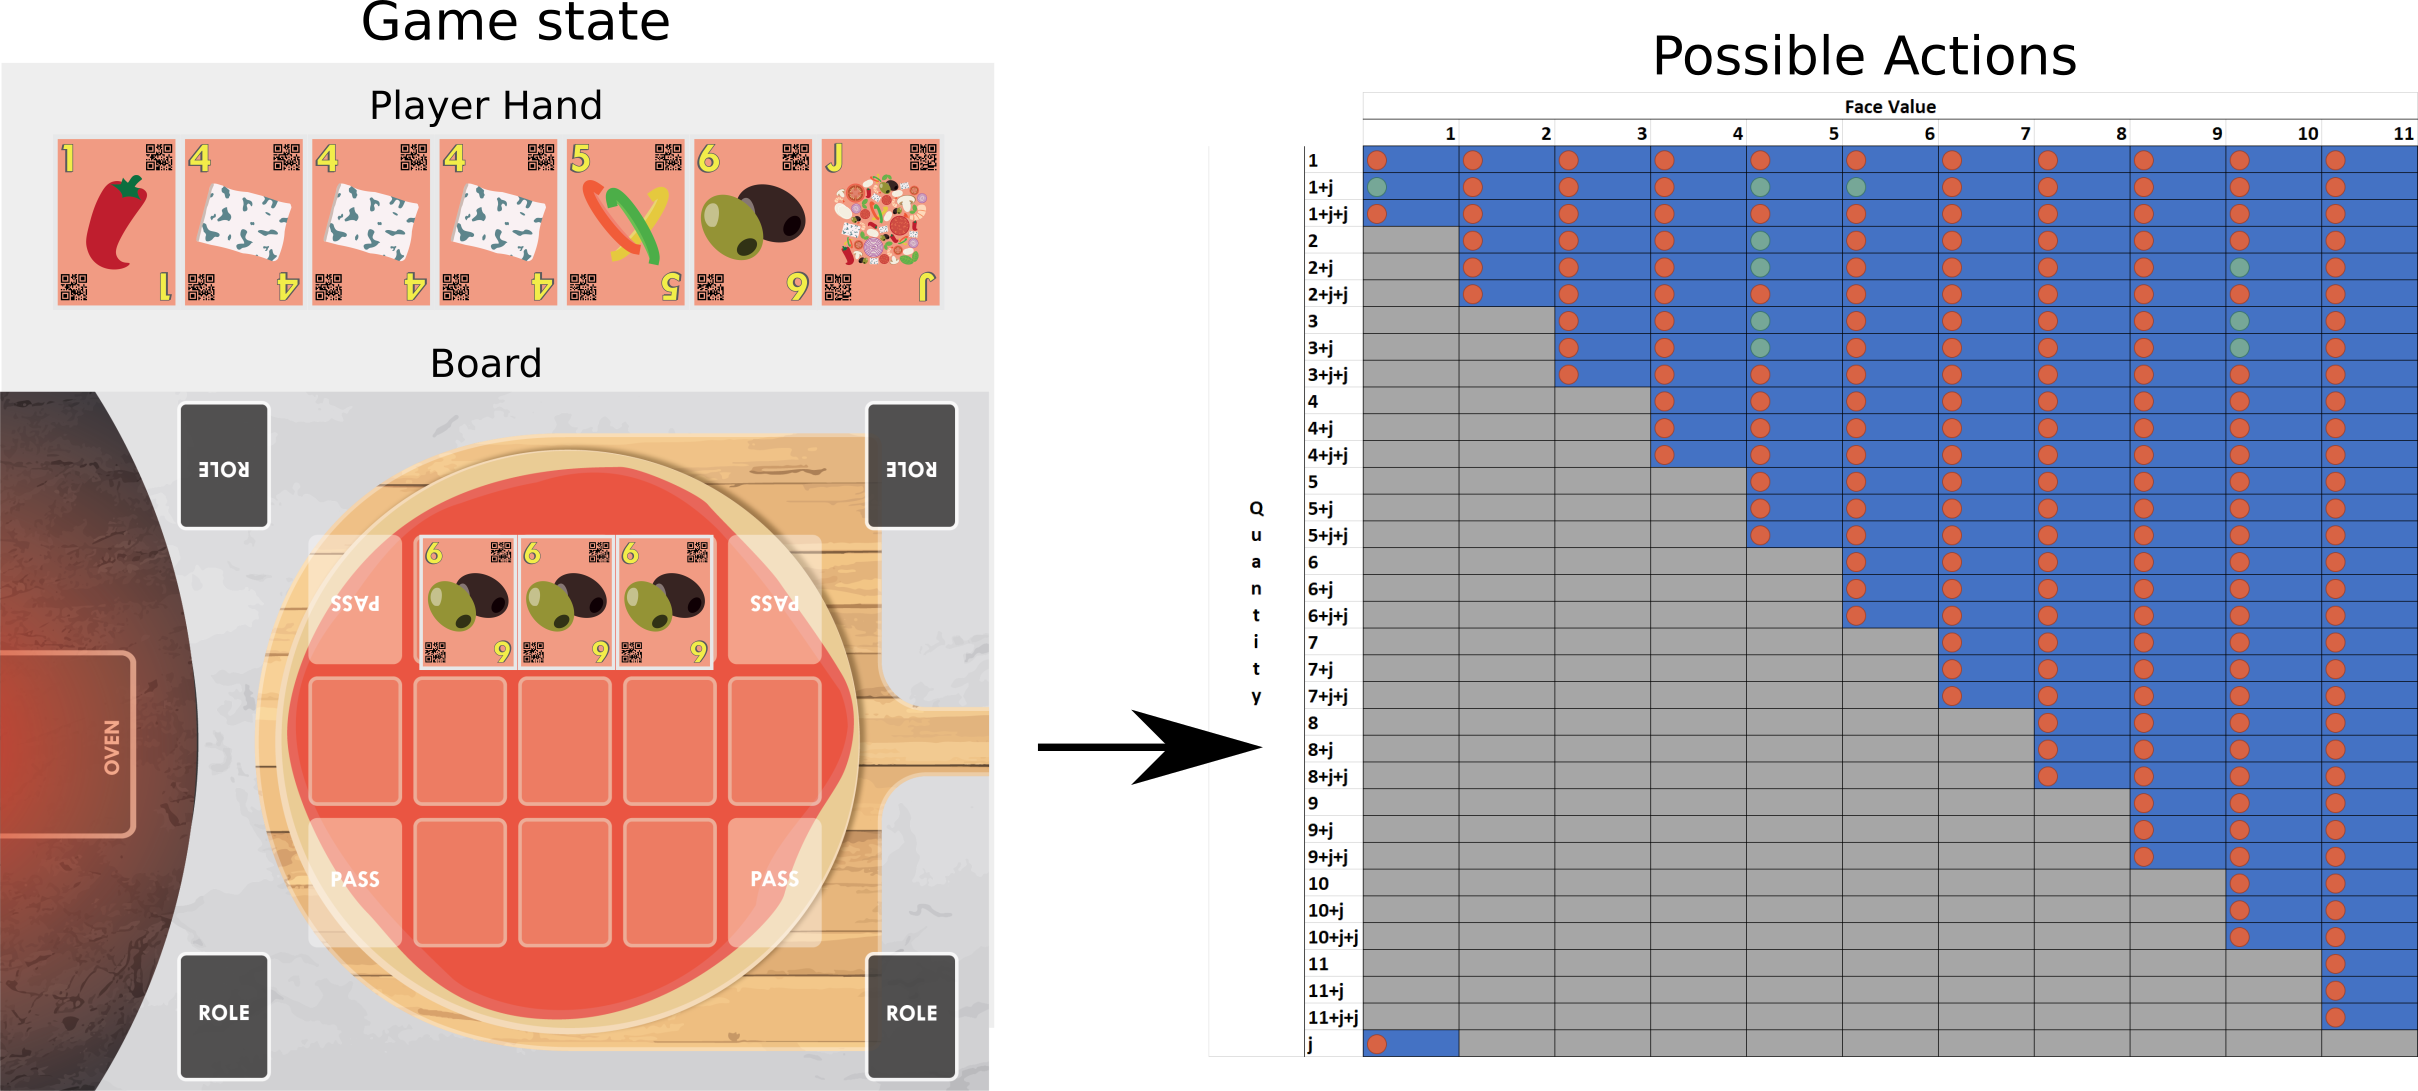
\includegraphics[width=1\columnwidth]{possibleActions.png}
    \caption{Example of possible actions given a certain game state. The columns represent the card face values, and the rows represent the number of cards to be discarded. The letter "j" represents the presence of a joker. It marks all the overall allowed actions (blue regions) and invalid actions(the gray regions), and the currently allowed actions (green dots).}
    \label{fig:possibleActions}
\end{figure}


\subsection{Q-Learning to the Rescue}

To train artificial agents to play Chef's Hat, we employ different reinforcement learning algorithms based on Q-learning. Q-Learning allows our agents to apply a temporal difference calculation when updating the policy network to maximize the state transitions that will lead to the optimal reward. In this regard, Q-learning showed a faster convergence and a simplified learning process \cite{shoham2003multi, gosavi2009reinforcement, kiumarsi2017optimal} when compared to other reinforcement learning methods. 

The general Q-learning algorithm learns to maximize the probability of choosing an action that leads to maximum reward. For that, it calculates a Q-value (quality value) for each action given a state and updates the policy, in our case represented by a neural network, to maximize the expected reward. Using a temporal difference calculation, it can take into consideration a sequence of steps that leads to the final state. In our simulation environment the final state is achieved when the player has no cards left in their hand. It gains maximal reward, once the player is the first one to reach the final state.

% The typical Q-learning algorithm represents a function $Q$ :

% \begin{equation}
% Q:SxA \rightarrow \mathbb{R}
% \end{equation}

% \noident where $S$ is the state, in our case represented by the 28 values composed by the cards at hand and the cards at the board. The actions, $A$, are expressed using the 200 discrete values for all the possible actions.

% To update the Q-values, the algorithm uses the following update function:

% \begin{equation}
%     Q'(s_t, a_t)= Q(s,a) + \alpha  \times \left (  TD \right )
% \end{equation}

% \noident where $\t$ is the current step, $\alpha$ is a pre-defined learning rate and $TD$ is the temporal difference function, calculated as:

% \begin{equation}
% TD =r_t \times \gamma \times maxQ\left (s__{t+1, a_t}  \right ) - maxQ\left (s__{t1, a_t}  \right )
% \end{equation}

% \noident where $r_t$ is the obtained reward for the state ($s_t$) and action ($a_t$) association, $\gamma$ represents the discount factor, a modulator that estimates the importance of the future rewards, and $maxQ\left (s__{t1, a_t}\right )$ is the estimate of Q-value for the next state.

\subsubsection{Chef's Hat Greedy Policy}

To provide an ideal balance between exploration and exploitation, an $\epsilon$-greedy exploration mechanism is usually adopted \cite{tokic2010adaptive, painter2012greedy, efroni2018multiple}. In the traditional form, each agent implements an action selection mechanism that ensures an exploration through random action selection at the beginning of the training:

\begin{equation}
a_t = \left\{\begin{matrix}
random(a) & if &  $x \leq \epsilon$\\ 
 Network(state))& if & $x > \epsilon$  
\end{matrix}\right.
\end{equation}

\noident where \emph{random(a)} represents a random action selection over the entire action space,  $\epsilon$ is the greedy factor, and $x$ a random number selected at each action. Usually $\epsilon$ starts with a higher value at the beginning of the training and it is reduced each time the policy is updated. This guarantees that the model performs a large number of exploratory steps at the beginning of the learning but incrementally starts to trust more and more on the policy update by the end of the learning phase.

In our scenario, however, performing a fully random action is not beneficial to the agent. As the game simulation only allows for valid actions to go through, and thus moving on towards the next game state, choosing random actions could lead to an agent getting stuck in a state until it chooses randomly a valid action. At the same time, penalizing the agent for choosing an invalid action is not ideal as it creates an unbalanced training set with a reward representing multiple goals: win the game, and perform valid actions, which creates unstable and unfocused learning. To solve this problem, we introduce here an updated greedy policy for the Chef's Hat agents. Instead of selecting a random action, the agent calculates the allowed actions given a state using Algorithm \ref{alg:possibleAction}.

\begin{algorithm}
 
 \State $PossibleActions\gets []$\\
 \State $JokersOnBoard\gets calculateJokersOnBoard()$\\
 \State $CardsInHand\gets cardsInHand()$\\
  \State $CardsInPlayingField\gets cardsInPlayField()$\\
  
  \State $firstAction \gets isFirstActionOfTheGame()$ \\
  
   \For{$CardValue\gets11$}{
        \For{$CardQuantity\gets11$}{
             \eIf{$CardValue$ in $CardsInHand$ and $CardValue \geq Max(cardsInPlayField)$}{
             
                 \eIf{$CardQuantity \leq CardsInHand[CardValue]$ and in $CardQuantity \geq Max(currentBoard) + JokersOnBoard$}{      
                 
                     \eIf{is $firstAction$}{
                         \eIf{$CardValue \eq 11$}{
                            \State  $PossibleActions \gets append(1)$
                         }
                         {
                          \State  $PossibleActions \gets append(0)$
                         }
                     
                      }
                      {
                        \State  $PossibleActions \gets append(1)$
                      }
    
                }
                {
                    \State  $PossibleActions \gets append(0)$
                }

                      
            }
            {
                \State  $PossibleActions \gets append(0)$
            }

         }
   }
    \KwResult{$PossibleActions$}\\
 
 \caption{Chef's Hat novel greedy action selection algorithm. It creates a vector containing all the 200 possible actions and which of them are allowed given a certain state.}
 \label{alg:possibleAction}
\end{algorithm}


The output of Algorithm \ref{alg:possibleAction} is hot-encoding with all the 200 possible actions, with a 1 representing an allowed action and a 0 representing an invalid actions given that specific state. Our $\epsilon$-greedy function is then represented by:

\begin{equation}
a_t = \left\{\begin{matrix}
random(PossibleActions(state)) & if &  $x \leq \epsilon$\\ 
 Network(state) & if & $x > \epsilon$  
\end{matrix}\right.
\end{equation}


\subsection{The Tale of Three Learners}

In order to validate our learning scenario and the Chef's Hat greedy action selection mechanism, we adapted three popular Q-learning-based methods: Deep Q-Learning - DQL \cite{van2016deep}, Advantage Actor-Critic - A2C \cite{mnih2016asynchronous}, and Proximal Policy Optimization - PPO \cite{schulman2017proximal}. Each of these algorithms represents one particular aspect of reinforcement learning, and our goal is to demonstrate how they learn and behave when deployed in our scenario using our specific greedy action selection process.

For each of the implemented algorithms, we use a mask composed of the output of Algorithm \ref{alg:possibleAction}. This mask is applied to the output layer that calculates the Q-values of the actions for each algorithm. The mask is extremely important as to guarantee that the output of the networks are in agreement with the games' mechanics, and thus, focus the Q-values maximization towards finding the best gameplay strategy.

All learning agents were optimized using a TPE optimization implemented by the Hyperopt \cite{bergstra2013hyperopt} library. Each of the learning agents implemented a single optimization routine for minimizing its loss when playing against dummy random agents. We implemented the agent using the Keras library \cite{gulli2017deep}, and our implementation is publicly available \footnote{https://github.com/pablovin/ChefsHatGYM}. 

\subsubsection{Deep Q-Learning}

\begin{figure}
    \centering
    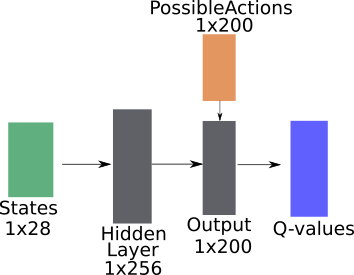
\includegraphics[width=0.7\columnwidth]{DQLNetwork.png}
    \caption{The DQL-based agent with a single network that learns to associate Q-values to a certain state.}
    \label{fig:dqlNetwork}
\end{figure}

Deep Q-learning is an evolution of the standard Q-learning method and introduces two novel aspects: a target model and the experience replay. The target model helps to stabilize the learning of Q by providing a stable Q-estimation over the training. The experience replay stores the agent's own experience by saving important steps taken by the agent, to increase the available data for learning state/action pairs through batch-learning. Deep Q-learning has been recently applied to teach agents to play complex video games with great success \cite{hausknecht2015deep, hester2018deep, meng2019qualitative}, mostly due to their capability of performing batch-learning using the experience replay. This increases drastically their training time but results in finding optimal game-winning strategies. We expect to see this behavior reflected on how this agent learns different strategies to play our game as well. Figure \ref{fig:dqlNetwork} illustrates the final architecture of the DQL agent.


% The target model introduces a second, the target model, policy which receives a snapshot of the original policy after a certain number of training steps.

% The target model is used to obtain the target Q learning when calculating the $TD_dql$:

% \begin{equation}
% TD_dql =r_t \times \gamma \times maxQ\left (s__{t+1, a_t}  \right ) - maxQ_t\left (s__{t1, a_t}  \right )
% \end{equation}

% \noident where $maxQ_t\left (s__{t1, a_t}  \right )$ is the Q-values obtained from the target network.

% The experience replay stores the agent's own experience by saving important steps taken by the agent, to increase the available data for learning state/action pairs through batch-learning. Deep Q-learning was recently applied to teach agents to play complex video games with great success \cite{hausknecht2015deep, hester2018deep, meng2019qualitative}. In our scenario, Q-learning has an advantage of updating the agent towards winning the game, and not only towards taking single-stepped actions. Figure \ref{fig:dqlNetwork} illustrates the final architecture of the DQL agent.


\subsubsection{Advantage Actor-Critic}

\begin{figure}
    \centering
    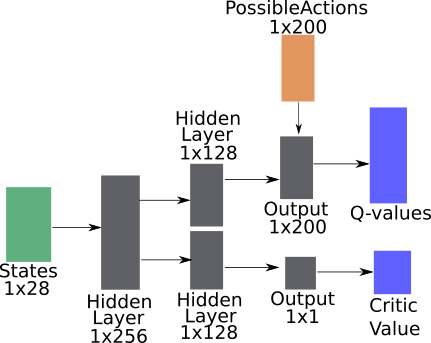
\includegraphics[width=0.8\columnwidth]{A2CNetwork.png}
    \caption{The A2C-based network presents a two-tailed implementation that encodes the state with a shared representation and decodes the Q-values and critic values using two separate outputs.}
    \label{fig:a2cNetwork}
\end{figure}

Actor-critic models present a hybrid learning method where an agent learns how to estimate the Q-values for a given state by following policy, the actor-network, and updates the chosen Q-values importance by a value-function approximator, the critic network. Advantage Action-critic \cite{mnih2016asynchronous} was introduced recently to stabilize the learning of the two networks by introducing the advantage function, which helps the entire model to identify given a certain state, how much better it is to take a specific action compared to the average action. Recent research demonstrates how A2C models present stable learning for video-games scenarios \cite{clary2019let}, and we expect to observe a steady improvement of this agent while learning a strategy. Our implementation of the A2C model uses a common decoder and a two-tailed network architecture and it is represented in Figure \ref{fig:a2cNetwork}. 


% Typical Action-Critic models are a on-policy learning methodology that learns how to measure a value for a policy while following it. This allows a stable online learning mechanism, where the model outputs the Q-values for an action, actor network, and independently, estimates a critic value about the actions selected by the actor using a critic network.

% \begin{equation}
% A(s_t,a_t) = r_t + \gamma \times V(s') - V(s)
% \end{equation}

% \noident where $V(s)$ represents the critic value for a given state, and $V(s')$ for the future state state. The advantage function is used to estabilizes training the actor network, while the critic network uses the discounted rewards as target. 


\subsubsection{PPO}


\begin{figure}
    \centering
    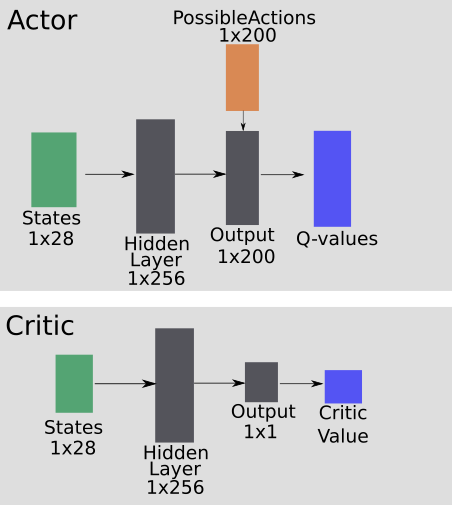
\includegraphics[width=0.7\columnwidth]{PPONetwork.png}
    \caption{Our PPO-based agent implements independent actor and critic networks, both receiving the state as input.}
    \label{fig:ppoNetwork}
\end{figure}

Our third implemented method is Proximal Policy Optimization (PPO) \cite{schulman2017proximal}. PPO is a recently introduced policy-based method, which follows the same learning structures as the A2C. It, however, implements an adaptive penalty control, based on the Kullback–Leibler divergence, to drive the updates of the agent at each interaction. This allows the model to create an update region that functions similarly to the stochastic gradient descent optimization, simplifying the necessity of the algorithm to keep large memory-replays or complex update rules. PPO has been used recently with great success in different competitive scenarios, where the environment is constantly changing  \cite{bansal2017emergent, kidzinski2018learning}. We expect that our PPO agent will present quick adaptation to newly perceived competitive strategies, in particular when playing against the other agents, which have a slower adaptation mechanism. The figure illustrates our PPO agent. Figure \ref{fig:ppoNetwork} illustrates the final model of our PPO agent.

\section{Evaluating Competition}

The goal of this paper is to demonstrate, evaluate and understand how the three reinforcement learning methods described above behave when learning in a competitive scenario provided by the Chef's Hat simulation environment. As such, we separate our evaluation routines into three experiments: First, we train one agent implementing each of these methods playing against three other agents implementing random action selections. Second, we perform a self-play training routine where each of the learning agents plays with different generations of themselves. Finally, we choose the best learning agent from the self-play experiments and play a competitive game with the three agents and a random agent.

\subsubsection{Reward and Metrics}

To train our agents we use an overall rewarding strategy: The environment gives a full reward when performing the action that leads an agent to win the game. Every other reward is set to -0.01. Given the temporal-difference learning, the agent will learn how to generate strategies, composed of a sequence of actions, to achieve the maximum reward, without receiving any prior information from the environment. 

For each experiment, we evaluate the agent's performance by calculating the networks' selected action Q-Values, the summed reward per game, and the total number of victories for all the games the agent played. The selected action Q-Values will give us an indication of how the confidence of agents in selecting actions behaves, while the summed reward will give us an overview of the overall performance of the agent over the entire game-span, combining victories and number of rounds. The total number of victories will indicate how well the agent is able to deal with the strategies of the other players. 

\subsection{vs Random}

Our first experiment puts each of the learning agents to play against three dummy agents. We perform a training routine that lasts 1000 games and measure the performance of the learning agents by plotting the evolution of the Q-value for the selected action and the summed reward for the entire training session. We then perform an evaluation routine where each trained agent plays 1000 games against the random agents, without further training and we measure the total of victories achieved by each agent. This experiment aims to give us important information about if each trained agent learns to beat a simple strategy based on random selections. Separating the training routine with a testing routine allows us to validate the learned strategies by the agents.

% The random agents are implemented to provide a random action selection based on the possible actions for each given state. Each learning agent is trained from scratch for 3000 games, meaning that at the beginning of the learning routine they will provide mostly random actions. Once they start learning, their behavior change. After each experiment, we run a test scenario where the trained agent plays 1000 games against the random agents, but without training. This allows us to validate the effectiveness of the learning procedure. The goal of this experiment is to demonstrate how each of the agents learns to devise winning strategies against random agents. 

\subsection{vs Myself}
Our second experiment is composed of a self-playing routine. For each self-play generation, we train agents playing against each other for 1000 games. In every generation, we save the best and second-best agents in a list, based on their summed reward when playing against each other in a validation routine: Without further training for 1000 games. For the next generation, we copy the best agent from the previous generation and put it to play against three other agents, which can be pulled from the best and second-best list, or a newly instantiated agent. The selection happens randomly, with the same probability of choosing any of these agents. We repeat the self-play routine for 50 generations, totaling 50.000 played games per learning method. We evaluate the impact of the self-playing routines by getting the first, the 25th and the last generation to play a game against the best agent from the previous experiment. We repeat this experiment for all three learning methods. This experiment allows us to observe how the self-playing routine affects the trained agents' performance within different generations.


% For each self-play generation, we train agents, with the same learning method, playing against each other for 1000 games. We then calculate the best agent by measuring their summed reward and re-start the routine by replacing the agents with the best agent. 

% We repeat this procedure for 10 generations, always copying the best agent of the previous generations to the new one.

% This experiment is composed of a self-play routine: we start the game with four agents implementing the same learning algorithm. After an initial experiment with 1000 games, we select the best agent, based on its summed reward output and start a new generation of agents which are initialized as a copy of the best agent. We run this experiment for 10 generations and provide a broad comparison of the performance of the agents' in-between generations.

\subsection{vs Others}

Our last experimental setup involves an inter-method evaluation. We take the best-trained agents for each learning method, based on the results of the vs Myself experiments, and put them to play against each other and a dummy agent. We perform two evaluation routines here: the first with these agents playing against each other for 1000 games, without further training. And the second with a training routine that lasts 3000 games followed by an evaluation routine that lasts 1000 games without training. This experiment will exhibit the performance of the implemented agents when compared to each other, and how they can adapt to more complex strategies than random action selection.

\subsection{Experimental Summary}

To better illustrate our entire experimental setup, we report all the experiments, training and validation routines, agent combinations and the number of games in Table \ref{tab:experimentalSetup}.

\begin{table}[h!]
\centering
\begin{tabular}{ c | c | c | c }
 \textbf{Exp.} & \textbf{Routine} & \textbf{Agents} &  \textbf{\# Games}\\ \hline
 \multirow{ 6}{*}{Random}  & \multirow{ 3}{*}{Train} & $1\times$ DQL vs $3\times$ Random & 1000 \\
   &&$1\times$ A2C vs $3\times$  Random & 1000 \\
   &&$1\times$ PPO vs $3\times$  Random & 1000 \\ \cline{2-4}
      & \multirow{ 3}{*}{Val.} & $1\times$ DQL vs $3\times$  Random & 1000 \\
   &&$1\times$ A2C vs $3\times$  Random & 1000 \\
   &&$1\times$ PPO vs $3\times$  Random & 1000 \\ \hline
   
  \multirow{ 6}{*}{Myself}  & \multirow{ 3}{*}{Train} & $4\times$ DQL & $1000\times50$ \\
   &&$4\times$ A2C & $1000\times50$ \\
   &&$4\times$ PPO & $1000\times50$ \\ \cline{2-4}
      & \multirow{ 3}{*}{Val.} &  $DQL_1$ vs $DQL_25$ vs $DQL_{50}$ vs $DQL_{r}$ & 1000 \\
   &&$A2C_1$ vs $A2C_25$ vs $A2C_{50}$ vs $A2C_{r}$ & 1000 \\
   &&$PPO_1$ vs $PPO_25$ vs $PPO_{50}$ vs $PPO_{r}$ & 1000 \\ \hline 
   
     \multirow{ 2}{*}{Others}  & Train. & DQL vs A2C vs PPO vs Random & 3000 \\\cline{2-4}
      & Val. &  DQL vs A2C vs PPO vs Random & 1000 \\ \hline 
  
%  Dense layer & 256 & ReLU \\
%  Dense layer & 200 & Tanh (output layer) \\\hline
%  Training Parameter & \multicolumn{2}{c}{Value}  \\ \hline
%  Batch Size & \multicolumn{2}{c}{ 32} \\
%  Memory size & \multicolumn{2}{c}{ 2000} \\  
%  discount rate & \multicolumn{2}{c}{ 0.95}  \\ 
%  exploration decay & \multicolumn{2}{c}{ 0.995} \\\hline   
 
\end{tabular}
\caption{Summary of our entire experimental setup, specifying our training and validation routines, agent combinations, and the number of performed games per routine.}
\label{tab:experimentalSetup}
\end{table}

\section{Results}
\subsection{vs Random}

Our Vs Random experiment results are illustrated in Figure \ref{fig:exp1Results}. We observe that, overall, the PPO agent is the one which presents the highest summed reward during the training phase, and the highest number of victories during the testing phase. As these experiments were performed against random agents, these numbers just inform us that all the agents learned how to beat a random strategy, with the PPO agent been the best on it. We explain this behavior due to the fast adaptation that the PPO learner provides, which makes it also achieves a higher overall summed reward, meaning it starts winning the random strategies quite earlier on when compared to the other two agents.  

\begin{figure}
    \centering
    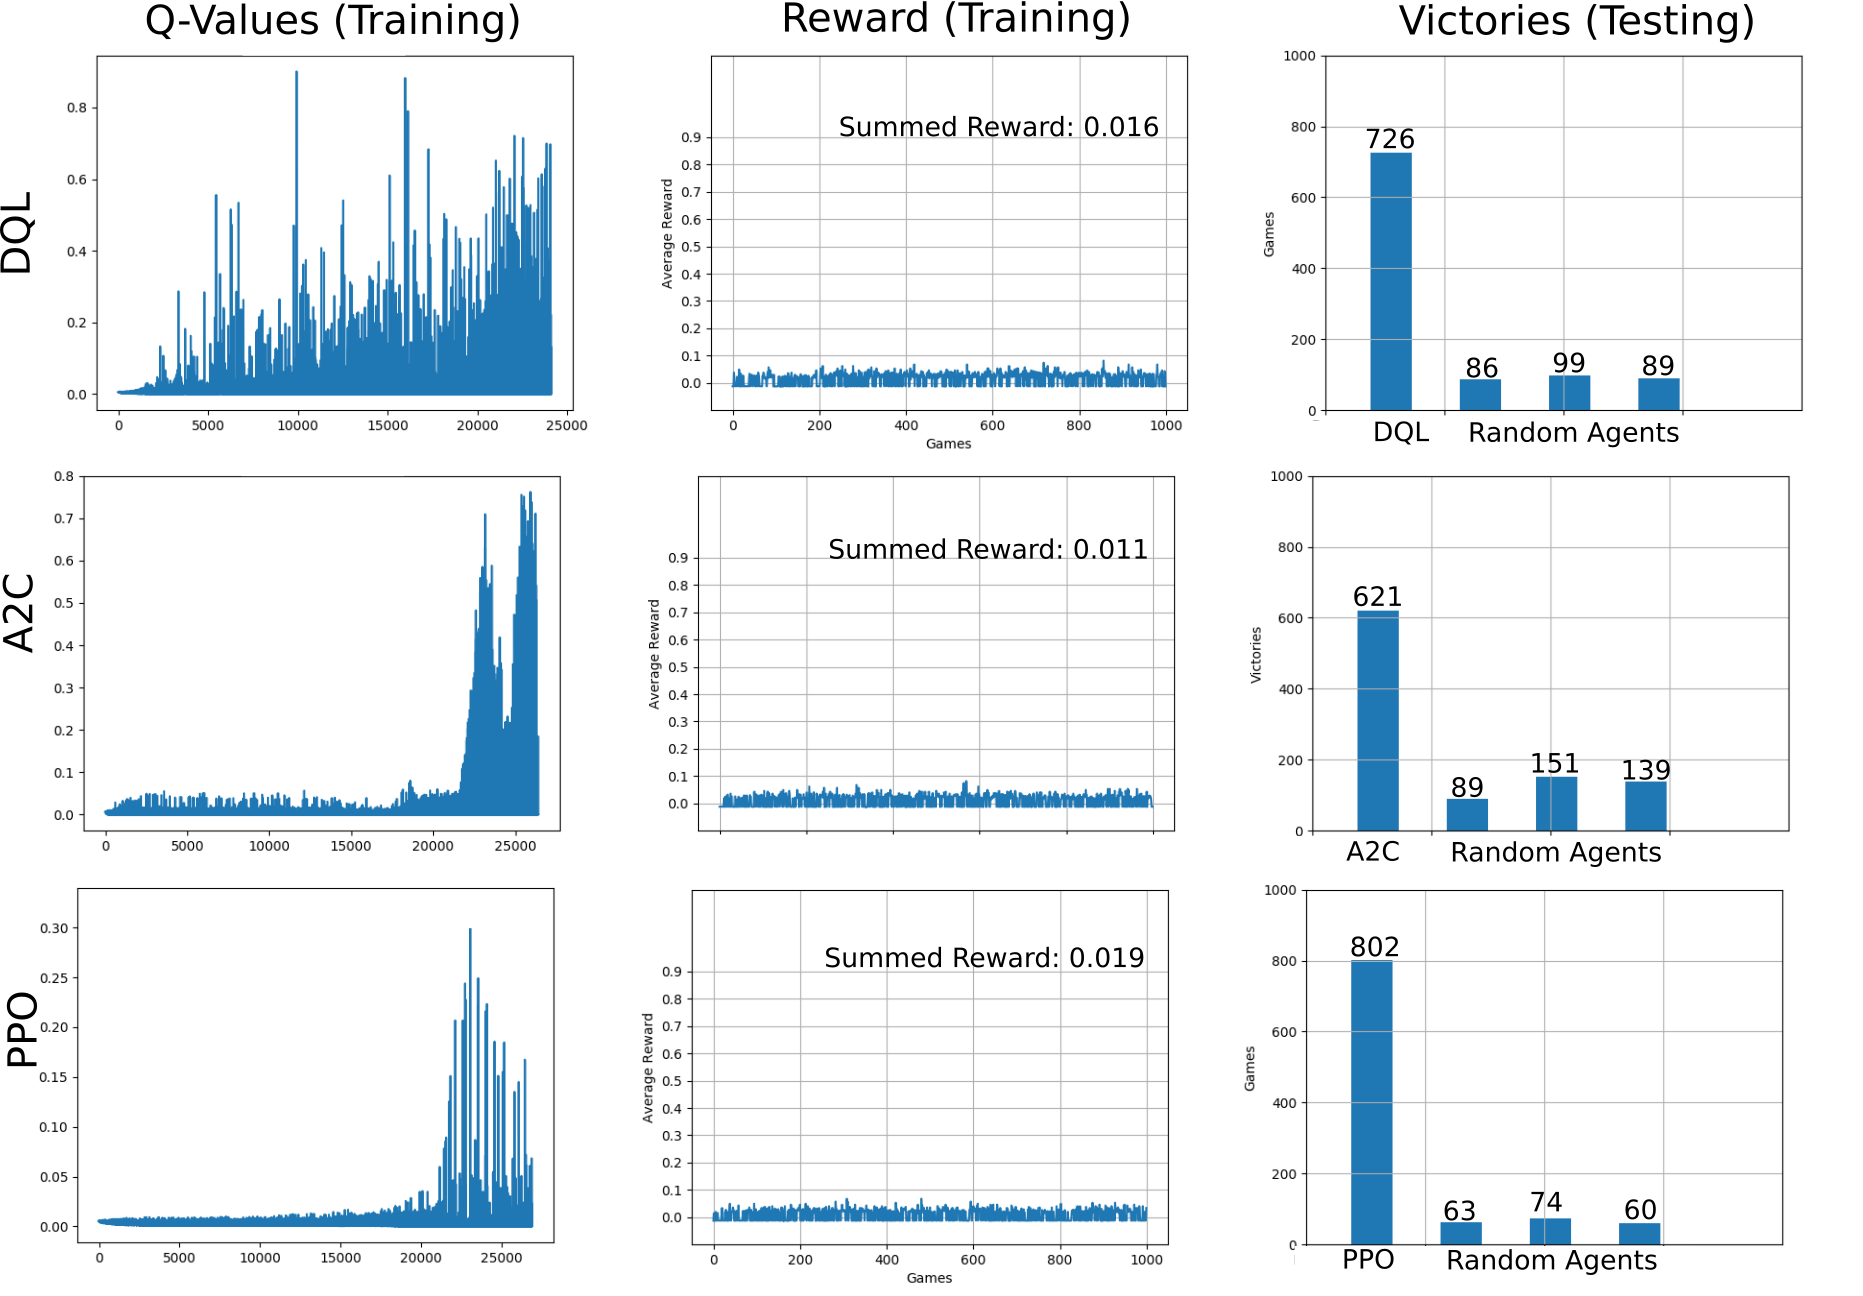
\includegraphics[width=1.0\columnwidth]{exp1Results.png}
    \caption{Exp.1 Results.}
    \label{fig:exp1Results}
\end{figure}

The Q-values evolution during training gives us an insight on when, during training, these agents start to select actions with higher confidence. While A2C and PPO agents take some games to provide higher confidence in the selected action, the DQL agent achieves a faster increase in confidence, starting already from the first games. This is probably due to the experience of replay-based training, which increases the number of state/action pairs that this agent is trained on per training routine. 

\subsection{vs Myself}
\subsection{vs Everyone else}

\section{What is to be competitive?}
\subsection{How do I learn the game?}
\subsection{How I learn competition?}
\subsection{How do I learn to be competitive?}

\section{Conclusion}



% conference papers do not normally have an appendix


% use section* for acknowledgment
%\section*{Acknowledgment}


%The authors would like to thank...





% trigger a \newpage just before the given reference
% number - used to balance the columns on the last page
% adjust value as needed - may need to be readjusted if
% the document is modified later
%\IEEEtriggeratref{8}
% The "triggered" command can be changed if desired:
%\IEEEtriggercmd{\enlargethispage{-5in}}

% references section

% can use a bibliography generated by BibTeX as a .bbl file
% BibTeX documentation can be easily obtained at:
% http://mirror.ctan.org/biblio/bibtex/contrib/doc/
% The IEEEtran BibTeX style support page is at:
% http://www.michaelshell.org/tex/ieeetran/bibtex/
%\bibliographystyle{IEEEtran}
% argument is your BibTeX string definitions and bibliography database(s)
%\bibliography{IEEEabrv,../bib/paper}
%
% <OR> manually copy in the resultant .bbl file
% set second argument of \begin to the number of references
% (used to reserve space for the reference number labels box)
\balance
\bibliographystyle{IEEEtran}
\bibliography{bib}





% that's all folks
\end{document}


